     \documentclass{article}

\usepackage{array}
\usepackage{etoolbox}
\usepackage{fancyhdr}
\usepackage{geometry}
\usepackage{graphicx}
\usepackage{soul}
\usepackage{titling}
\usepackage[english]{babel}
\usepackage[backend=biber]{biblatex}
\addbibresource{references.bib}
\usepackage{geometry}

% Set the page margins as per your requirement
\geometry{
  top=1in,
  bottom=1in,
  left=0.65in, % Increase the left margin
  right=0.65in, % Increase the right margin
}

%%%%%%%%%%%%%%%%%%%%%%%%%%%%%%%%%%%%%%%%%%%%%%%%%%%%%%%%%%%%
% BEGIN METADATA: Edit the following as appropriate
%%%%%%%%%%%%%%%%%%%%%%%%%%%%%%%%%%%%%%%%%%%%%%%%%%%%%%%%%%%%

\title{Bill-E}%Illuminating Pakistan's Electricity Consumption and Billing*%  % the title of your project
\newcommand\shorttitle{\thetitle}  % if needed: a shorter title for the document header
% Team members.
\newcommand\firstname{Ali Asghar Yousuf}  % full name
\newcommand\firstid{ay06993}         % ID, e.g. xy01234
\newcommand\secondname{Muhammad Azeem Haider} % full name
\newcommand\secondid{mh0658}        % ID, e.g. xy01234
\newcommand\thirdname{Mohammad Shahid Mahmood}  % full name
\newcommand\thirdid{mm06600}         % ID, e.g. xy01234
% Uncomment the rows for the next 2 students if and as needed.
\newcommand\fourthname{Syed Ibrahim Ali Haider} % full name
\newcommand\fourthid{sh06565}        % ID, e.g. xy01234
% \newcommand\fifthname{Student 5}  % full name
% \newcommand\fifthid{id05}         % ID, e.g. xy01234

%%%%%%%%%%%%%%%%%%%%%%%%%%%%%%%%%%%%%%%%%%%%%%%%%%%%%%%%%%%%
% END METADATA: Do not edit the preamble any further.
%%%%%%%%%%%%%%%%%%%%%%%%%%%%%%%%%%%%%%%%%%%%%%%%%%%%%%%%%%%%

\pagestyle{fancy}
\lhead{SRS}
\chead{\shorttitle}
\rhead{Fall 2023}
\cfoot{Page \thepage}
\renewcommand{\footrulewidth}{0.4pt}

\newcommand\instruction[1]{\textit{#1}}

\begin{document}

% Cover page.
\begin{titlepage}

\center % Center everything on the page
 
%----------------------------------------------------------------------------------------
%	HEADING SECTIONS
%----------------------------------------------------------------------------------------

\textsc{
  {\LARGE \bf \thetitle}\\\bigskip\bigskip % Your Project Title
  {\large
    Kaavish Software Requirements Specification\\\bigskip
    By}
}\\\bigskip 

%----------------------------------------------------------------------------------------
%	AUTHOR SECTION
%----------------------------------------------------------------------------------------

{\large
  \begin{tabular}{ll}
    \firstname & (\firstid@st.habib.edu.pk) \\
    \secondname & (\secondid@st.habib.edu.pk) \\
    \thirdname & (\thirdid@st.habib.edu.pk) \\
    \ifdef{\fourthname}{\fourthname & (\fourthid@st.habib.edu.pk) \\}{}
    \ifdef{\fifthname}{\fifthname & (\fifthid@st.habib.edu.pk) \\}{}
  \end{tabular}
}
\bigskip\bigskip\bigskip

{\large \today}\\\bigskip\bigskip


\includegraphics[height=5cm]{HU_logo}\\\bigskip
 
%----------------------------------------------------------------------------------------
{\large
  In partial fulfillment of the requirement for \\\medskip
Bachelor of Science \\\medskip
Computer Science
}\\\bigskip\bigskip\bigskip

{\large
  \textsc{
    Dhanani School of Science and Engineering\\\bigskip
    Habib University\\\bigskip 
    Fall 2023
  }\\\bigskip\bigskip 
  Copyright @ 2023 Habib University
}

\end{titlepage}


%%%%%%%%%%%%%%%%%%%%%%%%%%%%%%%%%%%%%%%%%%%%%%%%%%%%%%%%%%%%
% DATA: Populate the rest of the document as instructed.
%%%%%%%%%%%%%%%%%%%%%%%%%%%%%%%%%%%%%%%%%%%%%%%%%%%%%%%%%%%%
\section{Introduction}
% Write a clear and concise introduction explaining the purpose and scpe of the document.
This Software Requirements Specification Document is a blueprint for the development of our final year project's product, Bill-E, An electricity consumption and regulation App that aims to serve the public with insights about their electricity bill and the Units they consume over the course of a specified period. This document will outline the project plan, including the goals and objectives. It will also delve deep into the functional and non-functional requirements that we aim to meet whilst creating this software solution. It is intended for all the various stakeholders including the students, supervisors, testers, and end users, ensuring a common understanding of the scope and the behavior of the software.

\subsection{Purpose}
The primary purpose of this SRS is to define the functionality and features of the software and have a set of requirements in order to guide the development team. It will also help to plan, estimate, and allocate resources effectively. 

\subsection{Scope}
The scope of this document will cover the following key elements of Bill-E.
\begin{itemize}
    \item \textbf{Functionality and features:} A detailed description of the features and functionality of the application with a clear understanding of the software's expectations outlining the operations, interactions and capabilities that the stakeholders may experience.
    \item \textbf{Requirements Guidance} This SRS aims to establish an unambiguous set of requirements, which will serve as a guideline for the developers. These will include the functional and the non-functional requirements, as well as other important system requirements. All these are important for the designing, developing and testing of the software. 
    \item  \textbf{Project Planning and Resource Allocation:} By having a  clear set of requirements, The SRS will Aid the team in effectively planning the project, and allocate the required resources.
\end{itemize}
 
\section{Project Plan}
This section is where the different goals and objectives of the project are clearly stated and broken down into tasks. These tasks are then given a time frame and they are allotted the required resources. It is essential to have a project plan as it gives all the stakeholders, including student developers and supervisors a clear outline of the timelines and deliverables. An added part in this section are the risks that are involved in all the various part of the development journey of the project. 

\subsection{Objectives}
The objective of the Bill-E mobile application is to create a medium for users to predict their electricity consumption based on their previous/prior usage patterns. In addition, the application aims to provide recommendation to the users to reduce their electricity bill units. Providing users with analytics of their usage is another important work of the application. 

\subsection{Tasks}
the tasks
\subsection{Timelines}
the timelines

\subsection{Risks}
The risks involved with this project are as followed:

\begin{itemize}
    \item 
\end{itemize}


\section{Functional Requirements}
% Specify in detail the functions the software must perform.
todo: Provide a minimum of one use case representing different interactions with the system. \\ \\
Functional Requirements are a category of software requirements that describe what a software system or application is expected to do focusing on the interaction between the systems. These requirements detail the specific actions the software should be able to perform. this includes the inputs and the outputs, data processing, and user interface. They are essential for the design and development of the software. Following are a few of the main functions of our software, Bill-E.
\begin{itemize}
    \item \textbf{User Registration:} User will be able to create an account and delete an account.
    \item \textbf{User Input:} User will input data of past bills(in terms of units), current appliances, and usage hours, and a few other parameters related to billing, also giving them the option to update.
    \item \textbf{Room Breakdown:} User can add and remove rooms, according to their house structure.
    \item \textbf{Appliance Usage:} Users can add and remove the heavy, in-use appliances and their usage hours.
    \item \textbf{Update Appliance Usage:} User can update Appliance usage Hours.
    \item \textbf{Past Billing:} User will input the usage units of the past few months, for the accuracy of the prediction. 
    \item \textbf{User Profile Update:} The user can edit and update their profile.
    \item \textbf{Predict Consumption:} Users get their predicted electricity consumption based on the usage data provided.
    \item \textbf{Predicted Room Consumption:} Users get predicted room-wise consumption patterns.
    \item \textbf{Predict Bill:} Users get their predicted electricity consumption based on the usage data provided.
    \item \textbf{Recommendations:} Users can get recommendations regarding how to reduce their electricity consumption.
    \item \textbf{Analytics:} Users can look at the analytics regarding their consumption.
    \item \textbf{Highest Room Usage:} Users can look at the room that has consumed the most electricity.
    \item \textbf{Highest Usage Appliance:} Users can look at the Appliance that has consumed the most electricity.
    \item \textbf{Peak Consumption Time:} Users can look at their peak consumption time of electricity use.
    \item \textbf{Electricity Conservation Tips:} Users can view various conservation tips.
    \item \textbf{Bill Alerts:} User will be alerted if usage is projected to exceed a specific threshold just above the current slab rate.
    
\end{itemize}
    
    

\section{Non-Functional Requirements}

% Define performance e.g. security, reliability, scalability, usability, and compliance requirements for the software.
% Define specific examples for each type: performance, security, reliability, scalability, usability, and compliance requirements.
% Include additional non-functional requirements related to data integrity and backup
\begin{itemize}
    \item \textbf{Performance:} Predict usage within 5-10 seconds after running the input on the prediction model
    \item \textbf{Security:} Since the application will ask the users to input data on which prediction will occur, provide security so the data does not leak and users are not able to see other users' private data. 
    \item \textbf{Usability:} Intuitive UI for persons of every age group. eg. The app is not too complex that the functionality aspect is compromised at all
    \item \textbf{Compatibility:} The App will be compatible on both Android and IOS phones. 
    \item \textbf{Scalability:} 
    \item \textbf{Regulatory and Compliance:} We need to ensure that the App is aligned with all legal and industry regulations. 
    \item \textbf{Data Storage and Retention:} Ensure that the data collected is organized and after collection, it is secure, further used to enhance and improve the App and also backed up
\end{itemize}



\section{Usecase Diagram and Description}


\begin{figure}[h]
    \centering
    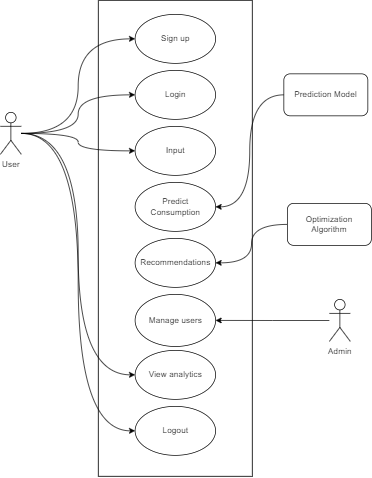
\includegraphics{usecase1.png}
    \caption{Use Case Diagram}
    \label{fig: Use Case Diagram}
\end{figure}
\textbf{Description:} The use case diagram serves the important purpose of visually giving a basic rundown of how the App will function for different Stakeholders. The Box indicates the boundary of the Applications and objects within the box are basically functional requirements of the application shown visually.
\begin{itemize}
    \item \textbf{Purpose: }
\end{itemize}


\section{System Diagram and Description:} 

% \section{References}
% \instruction{List your references.}
% \begin{itemize}
%     \item Amber, K. P., Ahmad, R., Farmanbar, M., Bashir, M. A., Mehmood, S., Khan, M. S., \& Saeed, M. U. (2021). Unlocking household electricity consumption in Pakistan. Buildings, 11(11), 566.
%     \item Lee, M. H. L., Ser, Y. C., Selvachandran, G., Thong, P. H., Cuong, L., Son, L. H., ... \& Gerogiannis, V. C. (2022). A comparative study of forecasting electricity consumption using machine learning models. Mathematics, 10(8), 1329.
%     \item Iftikhar, H., Bibi, N., Canas Rodrigues, P., \& López-Gonzales, J. L. (2023). Multiple Novel Decomposition Techniques for Time Series Forecasting: Application to Monthly Forecasting of Electricity Consumption in Pakistan. Energies, 16(6), 2579.
%     \item Predicting electricity energy consumption: A comparison of regression analysis, decision tree and neural networks
% \end{itemize}
\printbibliography


% External advisor undertaking.
%\begin{titlepage}

  \newcolumntype{C}[1]{>{\centering\arraybackslash\hspace{0pt}}p{#1}}

  \centerline{\textbf{\ul{Undertaking of Kaavish advisement as an External Supervisor}}}
  \bigskip\bigskip

  I hereby affirm that I have read the project details as described on the preceding pages and agree to undertake advisement of this Kaavish project as an External Supervisor. I understand that this role entails the following.
  \begin{description}
  \item[Meeting] Meeting the project team regularly, at least once every two weeks, for the entire duration of the Kaavish. The meetings may be held remotely if required.
  \item[Advisement] Providing supervision and advice to the team in order to ensure steady progress of the project toward its goals.
  \item[Liaison] Liaising with the Internal Supervisor as required, e.g. to provide feedback or engage in grading.
  \item[Other] Any other task, depending on availability and suitability, relevant to the Kaavish as communicated by the Internal Supervisor or Kaavish Working Group.
  \end{description}

  \bigskip\bigskip\bigskip
  
  \noindent
  \begin{tabular}{@{}lp{.4\textwidth}}
    Name: & \hrulefill\\\\
    Email: & \hrulefill\\\\
    Phone: & \hrulefill\\\\
    Designation: & \hrulefill\\\\
    Affiliation: & \hrulefill\\\\\\
    Signature: & \hrulefill\\
  \end{tabular}
\end{titlepage}


\end{document}

%%% Local Variables:
%%% mode: latex
%%% TeX-master: t
%%% End:
